\section{BaM}
\label{sec:chapter_4_section_1}
Il Progetto BaM (Building and Modelling) sviluppato in collaborazione con il CNG (Comitato Nazionale Geometri),
nasce dall'idea di far realizzare, agli studendi frequentanti le scuole medie in Italia,
l'\emph{aula che vorrei}. Lo scopo principale di questa iniziativa \'e sensibilizzare gli studenti a utilizzare
materiali ecosostenibili e rispettare l'ambiente.
Gli alunni avranno poi la possibilità di scegliere degli elementi con cui personalizzare l’aula virtuale.
La lista degli oggetti 3D presenti in libreria ha l’obiettivo di far sperimentare l’uso di uno strumento di progettazione
e di rappresentazione della realtà e di dare spunti su alcune tematiche di settore.\\
\\Per questo motivo il software è stato strutturato in modo che a ogni elemento è associato un punteggio su:
\begin{itemize}
\item impatto Ecologico;
\item impatto Energetico;
\item sicurezza;
\item rispetto della diversità/disabilità;
\end{itemize}
Vincerà il team che realizzerà la classe con il punteggio più alto, risultante dalla somma dei materiali scelti
tra quelli presenti in libreria. Per ottenere un punteggio alto, bisogna rispettare i principi delle
“3E” (Edilizia – Energia - Economia) e delle “3R” (Ridurre, Riutilizzare, Riciclare)!
\newpage

I plugins presenti all'interno del catalogo, sono stati suddivisi in categorie, per consentire una valutazione al
termine della realizzazione del modello dell'aula.
(come si evince dalle Figura~\ref{fig:figura1})...\\

\begin{figure}[htbp]
\begin{center}
\begin{tabular}{c @{\hspace{1em}} c}
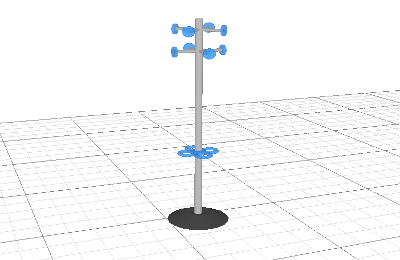
\includegraphics[width=5.5cm]{images/hanger} &
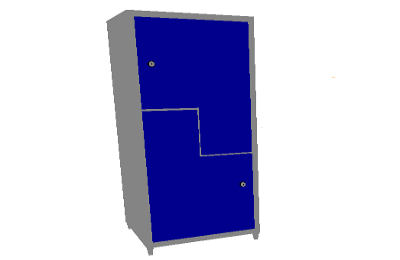
\includegraphics[width=5.5cm]{images/wardrobe} \\
 (a) & (b) \\
\end{tabular}
\begin{tabular}{c @{\hspace{1em}} c}
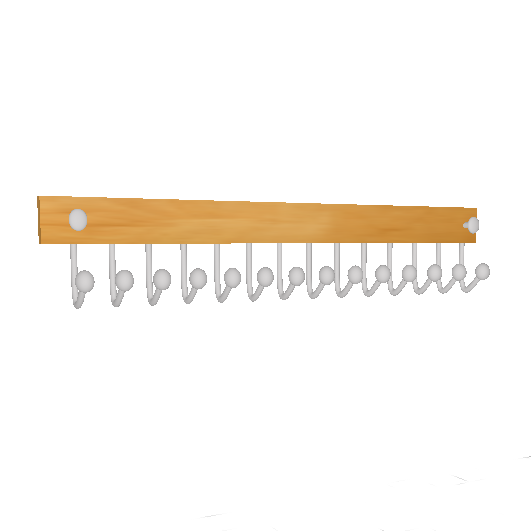
\includegraphics[width=5.5cm]{images/attaccapanni2} &
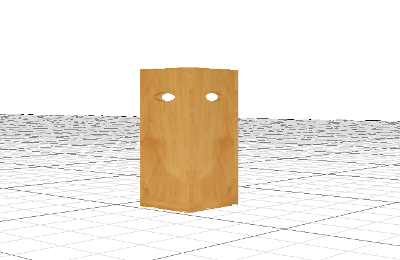
\includegraphics[width=5.5cm]{images/portaombrelli} \\
 (c) & (d) \\
\end{tabular}
\end{center}
\caption{Dettaglio Plugins: (a) appendiabiti, (b) armadietto, (c) attaccapanni, (d) portaombrelli}\label{fig:figura1}
\end{figure}
\newpage

TESTO RIEMPITIVO
Il Progetto BaM (Building and Modelling) sviluppato in collaborazione con il CNG (Comitato Nazionale Geometri),
nasce dall'idea di far realizzare, agli studendi frequentanti le scuole medie in Italia,
l'\emph{aula che vorrei}. Lo scopo principale di questa iniziativa \'e sensibilizzare gli studenti a utilizzare
materiali ecosostenibili e rispettare l'ambiente.

Come si evince dalle Figure~\ref{fig:figura2}

\begin{figure}[htbp]
\begin{center}
\begin{tabular}{c @{\hspace{1em}} c}
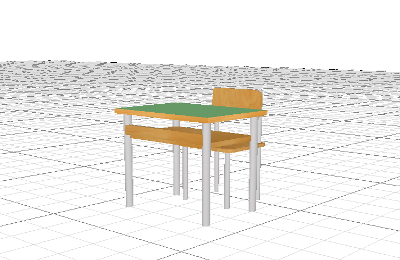
\includegraphics[width=5.5cm]{images/banco2} &
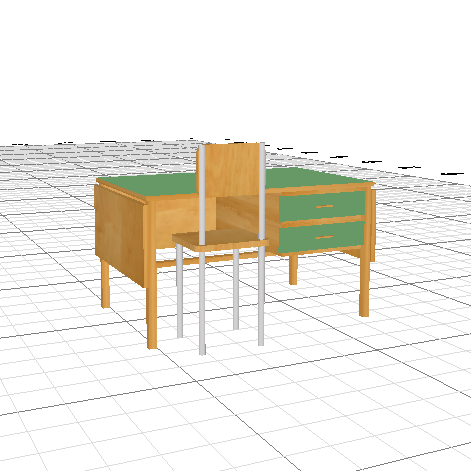
\includegraphics[width=5.5cm]{images/cattedra2} \\
 (a) & (b) \\
\end{tabular}
\begin{tabular}{c @{\hspace{1em}} c}
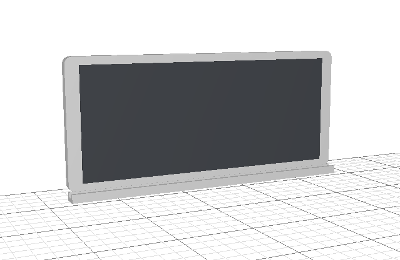
\includegraphics[width=5.5cm]{images/lavagna} &
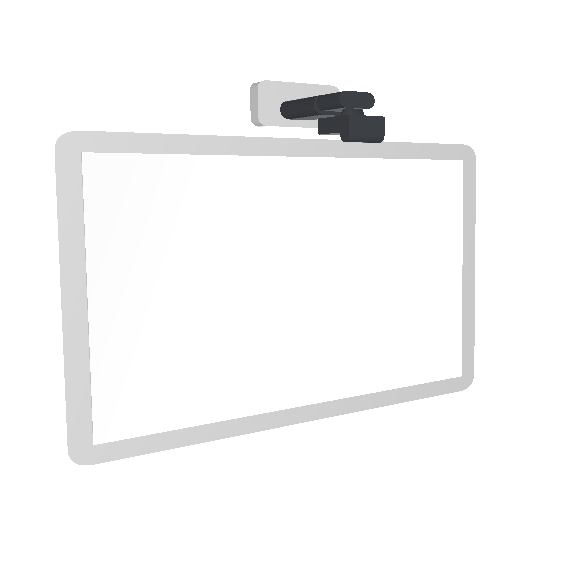
\includegraphics[width=5.5cm]{images/lim} \\
 (c) & (d) \\
\end{tabular}
\end{center}
\caption{Dettaglio Plugins: (a) banco, (b) cattedra, (c) lavagna, (d) lim}\label{fig:figura2}
\end{figure}
\newpage

TESTO RIEMPITIVO
Il Progetto BaM (Building And Modelling) sviluppato in collaborazione con il CNG (Comitato Nazionale Geometri),
nasce dall'idea di far realizzare, agli studendi frequentanti le scuole medie in Italia,
l'\emph{aula che vorrei}. Lo scopo principale di questa iniziativa \'e sensibilizzare gli studenti a utilizzare
materiali ecosostenibili e rispettare l'ambiente.

Come si evince dalle Figure~\ref{fig:figura3}


\begin{figure}[htbp]
\begin{center}
\begin{tabular}{c @{\hspace{1em}} c}
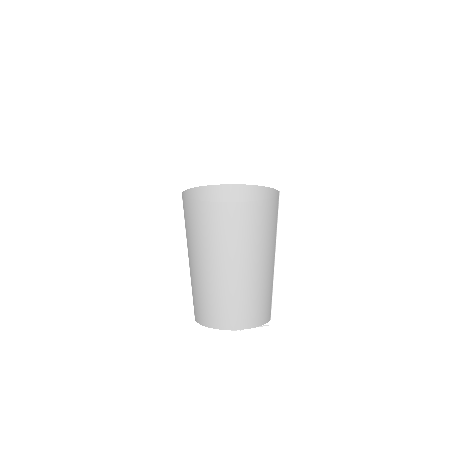
\includegraphics[width=5.5cm]{images/cestino} &
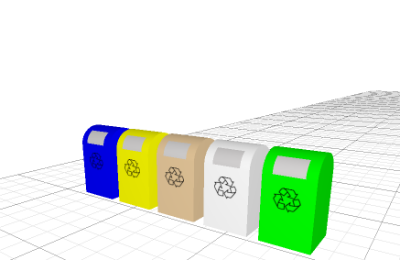
\includegraphics[width=5.5cm]{images/recycling-bins} \\
 (a) & (b) \\
\end{tabular}
\begin{tabular}{c @{\hspace{1em}} c}
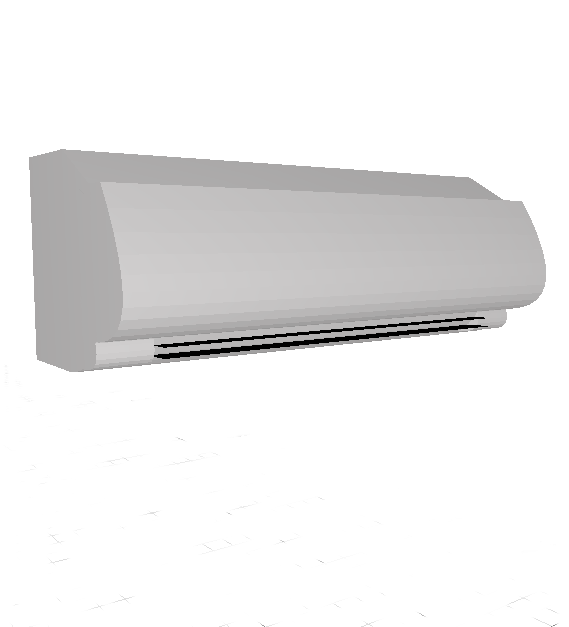
\includegraphics[width=5.5cm]{images/condizionatore} &
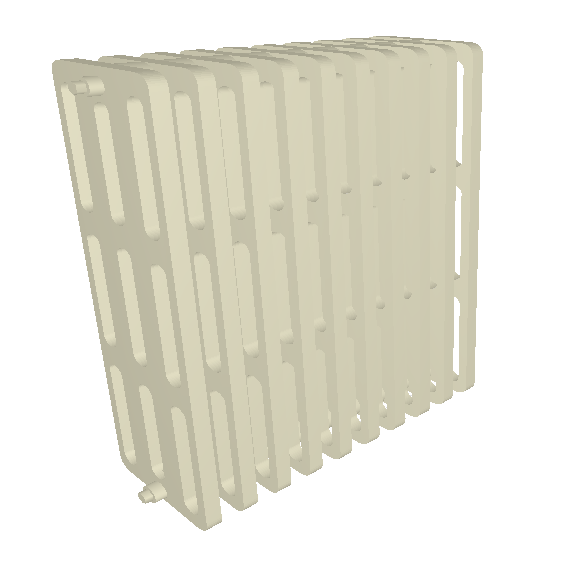
\includegraphics[width=5.5cm]{images/termosifone} \\
 (c) & (d) \\
\end{tabular}
\end{center}
\caption{Dettaglio Plugins: (a) cestino, (b) cestini differenziata, (c) condizionatore, (d) termosifone}\label{fig:figura3}
\end{figure}
\newpage

TESTO RIEMPITIVO
Il Progetto BAM (Building And Modelling) sviluppato in collaborazione con il CNG (Comitato Nazionale Geometri),
nasce dall'idea di far realizzare, agli studendi frequentanti le scuole medie in Italia,
l'\emph{aula che vorrei}. Lo scopo principale di questa iniziativa \'e sensibilizzare gli studenti a utilizzare
materiali ecosostenibili e rispettare l'ambiente.

Come si evince dalle Figure~\ref{fig:figura4}

\begin{figure}[htbp]
\begin{center}
\begin{tabular}{c @{\hspace{1em}} c}
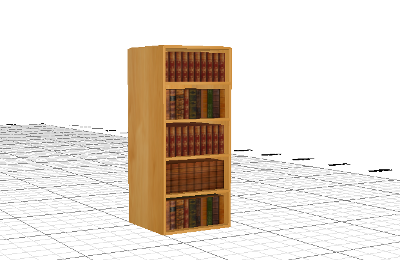
\includegraphics[width=5.5cm]{images/bookcase} &
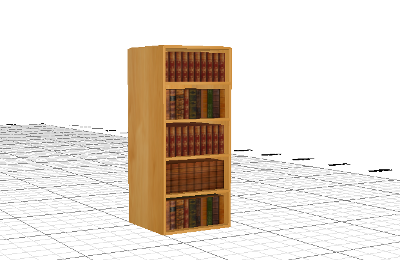
\includegraphics[width=5.5cm]{images/bookcase} \\
 (a) & (b) \\
\end{tabular}
\begin{tabular}{c @{\hspace{1em}} c}
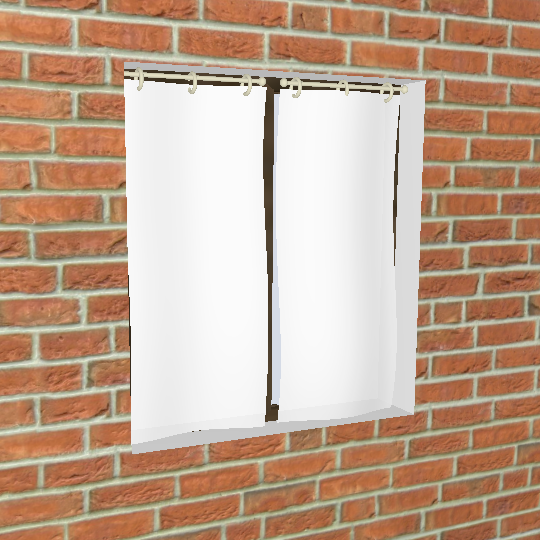
\includegraphics[width=5.5cm]{images/tenda} &
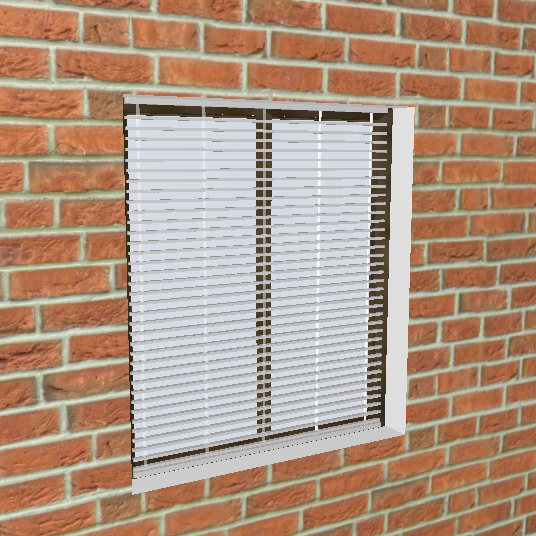
\includegraphics[width=5.5cm]{images/veneziana} \\
 (c) & (d) \\
\end{tabular}
\end{center}
\caption{Dettaglio Plugins: (a) libreria, (b) ???, (c) finestra con tenda, (d) finestra con veneziana}\label{fig:figura4}
\end{figure}

\newpage
